%%%%%%%%%%%%  Generated using docx2latex.pythonanywhere.com  %%%%%%%%%%%%%%


\documentclass[a4paper,12pt]{report}

% Other options in place of 'report' are 1)article 2)book 3)letter
% Other options in place of 'a4paper' are 1)a5paper 2)b5paper 3)letterpaper 4)legalpaper 5)executivepaper


 %%%%%%%%%%%%  Include Packages  %%%%%%%%%%%%%%


\usepackage{amsmath}
\usepackage{latexsym}
\usepackage{amsfonts}
\usepackage{amssymb}
\usepackage{graphicx}
\usepackage{txfonts}
\usepackage{wasysym}
\usepackage{enumitem}
\usepackage{adjustbox}
\usepackage{ragged2e}
\usepackage{tabularx}
\usepackage{changepage}
\usepackage{setspace}
\usepackage{hhline}
\usepackage{multicol}
\usepackage{float}
\usepackage{multirow}
\usepackage{makecell}
\usepackage{fancyhdr}
\usepackage[toc,page]{appendix}
\usepackage[utf8]{inputenc}
\usepackage[T1]{fontenc}
\usepackage{hyperref}


 %%%%%%%%%%%%  Define Colors For Hyperlinks  %%%%%%%%%%%%%%


\hypersetup{
colorlinks=true,
linkcolor=blue,
filecolor=magenta,
urlcolor=cyan,
}
\urlstyle{same}


 %%%%%%%%%%%%  Set Depths for Sections  %%%%%%%%%%%%%%

% 1) Section
% 1.1) SubSection
% 1.1.1) SubSubSection
% 1.1.1.1) Paragraph
% 1.1.1.1.1) Subparagraph


\setcounter{tocdepth}{5}
\setcounter{secnumdepth}{5}


 %%%%%%%%%%%%  Set Page Margins  %%%%%%%%%%%%%%


\usepackage[a4paper,bindingoffset=0.2in,headsep=0.5cm,left=1.0in,right=1.0in,bottom=2cm,top=2cm,headheight=2cm]{geometry}
\everymath{\displaystyle}


 %%%%%%%%%%%%  Set Depths for Nested Lists created by \begin{enumerate}  %%%%%%%%%%%%%%


\setlistdepth{9}
\newlist{myEnumerate}{enumerate}{9}
	\setlist[myEnumerate,1]{label=\arabic*)}
	\setlist[myEnumerate,2]{label=\alph*)}
	\setlist[myEnumerate,3]{label=(\roman*)}
	\setlist[myEnumerate,4]{label=(\arabic*)}
	\setlist[myEnumerate,5]{label=(\Alph*)}
	\setlist[myEnumerate,6]{label=(\Roman*)}
	\setlist[myEnumerate,7]{label=\arabic*}
	\setlist[myEnumerate,8]{label=\alph*}
	\setlist[myEnumerate,9]{label=\roman*}

\renewlist{itemize}{itemize}{9}
	\setlist[itemize]{label=$\cdot$}
	\setlist[itemize,1]{label=\textbullet}
	\setlist[itemize,2]{label=$\circ$}
	\setlist[itemize,3]{label=$\ast$}
	\setlist[itemize,4]{label=$\dagger$}
	\setlist[itemize,5]{label=$\triangleright$}
	\setlist[itemize,6]{label=$\bigstar$}
	\setlist[itemize,7]{label=$\blacklozenge$}
	\setlist[itemize,8]{label=$\prime$}



 %%%%%%%%%%%%  Header here  %%%%%%%%%%%%%%


\pagestyle{fancy}
\fancyhf{}


 %%%%%%%%%%%%  Footer here  %%%%%%%%%%%%%%




 %%%%%%%%%%%%  Print Page Numbers  %%%%%%%%%%%%%%


\rfoot{\thepage}


 %%%%%%%%%%%%  This sets linespacing (verticle gap between Lines) Default=1 %%%%%%%%%%%%%%


\setstretch{1.08}


 %%%%%%%%%%%%  Document Code starts here %%%%%%%%%%%%%%


\begin{document}
\sloppy
\begin{center}{\fontsize{24pt}{24pt}\selectfont \textbf{Python Exceptions Handling} 

 %%%%%%%%%%%%  Figure/Image No:1 here %%%%%%%%%%%%%%


\begin{figure}[H]
\begin{center}
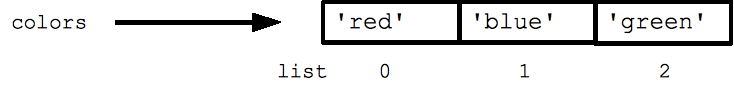
\includegraphics[width=6.84in,height=5.14in]{./uploads_new/Python_Exceptions_Handling.docx_DIR/media/image1.jpeg}
\end{center}
\end{figure}


 %%%%%%%%%%%%  Figure/Image No:1 Ends Here %%%%%%%%%%%%%%


 \\}\end{center} \par
\noindent 
Python menyediakan dua fitur yang sangat penting untuk menangani kesalahan tak terduga dalam program Python Anda dan menambahkan kemampuan debugging di dalamnya - \par
\noindent 
\vspace{12pt}
\noindent 
 $  $ $  $ $  $ $  $Exception Handling: Ini akan dibahas dalam tutorial ini. Berikut adalah daftar standar Pengecualian yang tersedia dengan Python: Pengecualian Standar. \par
\noindent 
\vspace{12pt}
\noindent 
 $  $ $  $ $  $ $  $Penegasan: Ini akan dibahas dalam Asertions dengan tutorial Python. \par
\noindent 
\vspace{12pt}
\noindent 
Daftar Pengecualian Standar – \par
\noindent 
\vspace{12pt}


 %%%%%%%%%%%%  Table No:1 Here %%%%%%%%%%%%%%


\begin{table}[H]
\centering
\begin{adjustbox}{width=\textwidth}
\begin{tabular}{ p{1.77in}p{4.49in} }
\hhline{--}
\multicolumn{1}{|p{1.77in}}{\Centering EXCEPTION NAME} & \multicolumn{1}{|p{4.49in}|}{\Centering DESCRIPTION} & \hhline{--}
\multicolumn{1}{|p{1.77in}}{Exception} & \multicolumn{1}{|p{4.49in}|}{Kelas dasar untuk semua pengecualian} & \hhline{--}
\multicolumn{1}{|p{1.77in}}{StopIteration} & \multicolumn{1}{|p{4.49in}|}{Dibesarkan ketika metode (iterator) berikutnya dari iterator tidak mengarah ke objek apa pun.} & \hhline{--}
\multicolumn{1}{|p{1.77in}}{SystemExit} & \multicolumn{1}{|p{4.49in}|}{Dibesarkan oleh fungsi sys.exit ().} & \hhline{--}
\multicolumn{1}{|p{1.77in}}{StandardError} & \multicolumn{1}{|p{4.49in}|}{Kelas dasar untuk semua pengecualian built-in kecuali StopIteration dan SystemExit} & \hhline{--}
\multicolumn{1}{|p{1.77in}}{ArithmeticError} & \multicolumn{1}{|p{4.49in}|}{Kelas dasar untuk semua kesalahan yang terjadi untuk perhitungan numerik.} & \hhline{--}
\multicolumn{1}{|p{1.77in}}{OverflowError} & \multicolumn{1}{|p{4.49in}|}{Dibesarkan saat perhitungan melebihi batas maksimum untuk tipe numerik.} & \hhline{--}
\multicolumn{1}{|p{1.77in}}{FloatingPointError} & \multicolumn{1}{|p{4.49in}|}{Dibesarkan saat perhitungan floating point gagal.} & \hhline{--}
\multicolumn{1}{|p{1.77in}}{ZeroDivisionError} & \multicolumn{1}{|p{4.49in}|}{Dibesarkan saat pembagian atau modulo nol dilakukan untuk semua tipe numerik.} & \hhline{--}
\multicolumn{1}{|p{1.77in}}{AssertionError} & \multicolumn{1}{|p{4.49in}|}{Dibesarkan jika terjadi kegagalan pernyataan Assert.} & \hhline{--}
\multicolumn{1}{|p{1.77in}}{AttributeError} & \multicolumn{1}{|p{4.49in}|}{Dibesarkan jika terjadi kegagalan referensi atribut atau penugasan.} & \hhline{--}
\multicolumn{1}{|p{1.77in}}{EOFError} & \multicolumn{1}{|p{4.49in}|}{Dibesarkan bila tidak ada input dari fungsi raw $  \_  $input () atau input () dan akhir file tercapai.} & \hhline{--}
\multicolumn{1}{|p{1.77in}}{ImportError} & \multicolumn{1}{|p{4.49in}|}{Dibesarkan saat sebuah pernyataan impor gagal.} & \hhline{--}
\multicolumn{1}{|p{1.77in}}{KeyboardInterrupt} & \multicolumn{1}{|p{4.49in}|}{Dibesarkan saat pengguna menyela eksekusi program, biasanya dengan menekan Ctrl + c.} & \hhline{--}
\multicolumn{1}{|p{1.77in}}{LookupError} & \multicolumn{1}{|p{4.49in}|}{Kelas dasar untuk semua kesalahan pencarian.} & \hhline{--}
\multicolumn{1}{|p{1.77in}}{IndexErrorKeyError} & \multicolumn{1}{|p{4.49in}|}{Dibesarkan saat sebuah indeks tidak ditemukan secara berurutan.Dibesarkan saat kunci yang ditentukan tidak ditemukan dalam kamus.} & \hhline{--}
\multicolumn{1}{|p{1.77in}}{NameError} & \multicolumn{1}{|p{4.49in}|}{Dibesarkan saat pengenal tidak ditemukan di namespace lokal atau global.} & \hhline{--}
\multicolumn{1}{|p{1.77in}}{UnboundLocalErrorEnvironmentError} & \multicolumn{1}{|p{4.49in}|}{Dibesarkan saat mencoba mengakses variabel lokal dalam suatu fungsi atau metode namun tidak ada nilai yang ditugaskan padanya.Kelas dasar untuk semua pengecualian yang terjadi di luar lingkungan Python.} & \hhline{--}
\multicolumn{1}{|p{1.77in}}{IOErrorIOError} & \multicolumn{1}{|p{4.49in}|}{Dibesarkan saat operasi input / output gagal, seperti pernyataan cetak atau fungsi open () saat mencoba membuka file yang tidak ada.Dibangkitkan untuk kesalahan terkait sistem operasi.} & \hhline{--}
\multicolumn{1}{|p{1.77in}}{SyntaxErrorIndentationError} & \multicolumn{1}{|p{4.49in}|}{Dibesarkan saat ada kesalahan dengan sintaks Python.Dibesarkan saat indentasi tidak ditentukan dengan benar.} & \hhline{--}
\multicolumn{1}{|p{1.77in}}{SystemError} & \multicolumn{1}{|p{4.49in}|}{Dibesarkan saat penafsir menemukan masalah internal, namun bila kesalahan ini ditemui juru bahasa Python tidak keluar.} & \hhline{--}
\multicolumn{1}{|p{1.77in}}{SystemExit} & \multicolumn{1}{|p{4.49in}|}{Dibesarkan saat juru bahasa Python berhenti dengan menggunakan fungsi sys.exit (). Jika tidak ditangani dalam kode, menyebabkan penafsir untuk keluar.} & \hhline{--}
\multicolumn{1}{|p{1.77in}}{TypeError} & \multicolumn{1}{|p{4.49in}|}{Dibesarkan saat operasi atau fungsi dicoba yang tidak valid untuk tipe data yang ditentukan.} & \hhline{--}
\multicolumn{1}{|p{1.77in}}{ValueError} & \multicolumn{1}{|p{4.49in}|}{Dibesarkan saat fungsi bawaan untuk tipe data memiliki jenis argumen yang valid, namun argumen tersebut memiliki nilai yang tidak valid yang ditentukan.} & \hhline{--}
\multicolumn{1}{|p{1.77in}}{RuntimeError} & \multicolumn{1}{|p{4.49in}|}{Dibesarkan saat kesalahan yang dihasilkan tidak termasuk dalam kategori apa pun.} & \hhline{--}
\multicolumn{1}{|p{1.77in}}{NotImplementedError} & \multicolumn{1}{|p{4.49in}|}{Dibesarkan ketika metode abstrak yang perlu diimplementasikan di kelas warisan sebenarnya tidak diimplementasikan} & \hline
\end{tabular}
\end{adjustbox}
\end{table}


 %%%%%%%%%%%%  Table No:1 Ends Here %%%%%%%%%%%%%%


\noindent 
\vspace{12pt}
\noindent 
Penegasan dengan Python \par
\vspace{12pt}
\noindent 
Penegasan adalah pemeriksaan kewarasan yang dapat Anda aktifkan atau matikan saat Anda selesai dengan pengujian program Anda. \par
\vspace{12pt}
\noindent 
Cara termudah untuk memikirkan sebuah pernyataan adalah menyamakannya dengan pernyataan kenaikan gaji-jika (atau lebih akurat, pernyataan kenaikan-jika-tidak). Sebuah ekspresi diuji, dan jika hasilnya muncul salah, pengecualian akan meningkat. \par
\vspace{12pt}
\noindent 
Penegasan dilakukan dengan pernyataan tegas, kata kunci terbaru untuk Python, diperkenalkan di versi 1.5. \par
\vspace{12pt}
\noindent 
Pemrogram sering menempatkan asersi pada awal fungsi untuk memeriksa masukan yang valid, dan setelah pemanggilan fungsi untuk memeriksa keluaran yang valid. \par
\noindent 
Pernyataan tegas \par
\vspace{12pt}
\noindent 
Ketika menemukan pernyataan tegas, Python mengevaluasi ekspresi yang menyertainya, yang semoga benar. Jika ungkapannya salah, Python menimbulkan pengecualian AssertionError. \par
\vspace{12pt}
\noindent 
Sintaks untuk menegaskan adalah - \par
\vspace{12pt}
\noindent 
menegaskan Ekspresi [, Argumen] \par
\vspace{12pt}
\noindent 
Jika asersi gagal, Python menggunakan ArgumentExpression sebagai argumen untuk AssertionError. Penegasan Pengecualian pengecualian dapat ditangkap dan ditangani seperti pengecualian lainnya dengan menggunakan perintah try-except, namun jika tidak ditangani, mereka akan menghentikan program dan menghasilkan traceback. \par
\noindent 
Contoh \par
\vspace{12pt}
\noindent 
Berikut adalah fungsi yang mengubah suhu dari derajat Kelvin sampai derajat Fahrenheit. Karena nol derajat Kelvin sedingin yang didapatnya, fungsi itu mundur jika melihat suhu negatif - \par
\noindent 
 $  \#  $!/usr/bin/python \par
\noindent 
def KelvinToFahrenheit(Temperature): \par
\noindent 
~~ assert (Temperature >= 0),"Colder than absolute zero!" \par
\noindent 
~~ return ((Temperature-273)*1.8)+32 \par
\noindent 
print KelvinToFahrenheit(273) \par
\noindent 
print int(KelvinToFahrenheit(505.78)) \par
\noindent 
print KelvinToFahrenheit(-5) \par
\vspace{14pt}
\noindent 
Bila kode diatas dieksekusi, maka menghasilkan hasil sebagai berikut – \par
\noindent 
32.0 \par
\noindent 
451 \par
\noindent 
Traceback (most recent call last): \par
\noindent 
File "test.py", line 9, in  \par
\noindent 
print KelvinToFahrenheit(-5) \par
\noindent 
File "test.py", line 4, in KelvinToFahrenheit \par
\noindent 
assert (Temperature >= 0),"Colder than absolute zero!" \par
\noindent 
AssertionError: Colder than absolute zero! \par
\vspace{12pt}
\vspace{12pt}
\noindent 
Apa itu Exception? \par
\vspace{12pt}
\noindent 
Pengecualian adalah sebuah peristiwa, yang terjadi selama pelaksanaan program yang mengganggu aliran normal instruksi program. Secara umum, ketika skrip Python menemukan situasi yang tidak dapat diatasi, hal itu menimbulkan pengecualian. Pengecualian adalah objek Python yang mewakili kesalahan. \par
\vspace{12pt}
\noindent 
Ketika skrip Python menimbulkan pengecualian, ia harus menangani pengecualian begitu saja sehingga berhenti dan berhenti. \par
\noindent 
Menangani pengecualian \par
\vspace{12pt}
\noindent 
Jika Anda memiliki beberapa kode yang mencurigakan yang mungkin menimbulkan pengecualian, Anda dapat mempertahankan program Anda dengan menempatkan kode yang mencurigakan di coba: blokir. Setelah dicoba: blokir, sertakan sebuah pernyataan kecuali:, diikuti oleh blok kode yang menangani masalah ini seaman mungkin. \par
\noindent 
Sintaksis \par
\vspace{12pt}
\noindent 
Berikut adalah sintaks sederhana coba .... kecuali ... blok lain – \par
\vspace{12pt}
\noindent 
try: \par
\noindent 
~~ You do your operations here; \par
\noindent 
~~ ...................... \par
\noindent 
except \textit{ExceptionI}: \par
\noindent 
~~ If there is ExceptionI, then execute this block. \par
\noindent 
except \textit{ExceptionII}: \par
\noindent 
~~ If there is ExceptionII, then execute this block. \par
\noindent 
~~ ...................... \par
\noindent 
else: \par
\noindent 
~~ If there is no exception then execute this block \par
\vspace{12pt}
\vspace{12pt}
\noindent 
Berikut adalah beberapa poin penting tentang sintaks yang disebutkan di atas - \par
\vspace{12pt}
\noindent 
 $  $ $  $ $  $ $  $Pernyataan percobaan tunggal dapat memiliki banyak kecuali pernyataan. Ini berguna saat blok coba berisi pernyataan yang mungkin membuang berbagai jenis pengecualian. \par
\vspace{12pt}
\noindent 
 $  $ $  $ $  $ $  $Anda juga bisa memberikan klausa umum kecuali klausul, yang menangani pengecualian apapun. \par
\vspace{12pt}
\noindent 
 $  $ $  $ $  $ $  $Setelah klausa kecuali, Anda bisa memasukkan klausul lain. Kode di blok yang lain dijalankan jika kode di coba: blok tidak menimbulkan pengecualian. \par
\vspace{12pt}
\noindent 
 $  $ $  $ $  $ $  $Blok yang lain adalah tempat yang baik untuk kode yang tidak perlu dicoba: perlindungan blokir. \par
\vspace{12pt}
\noindent 
Contoh \par
\vspace{12pt}
\noindent 
Contoh ini membuka file, menulis konten di file, dan keluar dengan anggun karena tidak ada masalah sama sekali - \par
\vspace{16pt}
\noindent 
 $  \#  $!/usr/bin/python \par
\vspace{12pt}
\noindent 
try: \par
\noindent 
~~ fh = open("testfile", "w") \par
\noindent 
~~ fh.write("This is my test file for exception handling!!") \par
\noindent 
except IOError: \par
\noindent 
~~ print "Error: can $  \textbackslash  $'t find file or read data" \par
\noindent 
else: \par
\noindent 
~~ print "Written content in the file successfully" \par
\noindent 
~~ fh.close() \par
\vspace{16pt}
\noindent 
Ini menghasilkan hasil sebagai berikut - \par
\vspace{12pt}
\noindent 
Written content in the file successfully \par
\vspace{12pt}
\noindent 
Klausul kecuali tanpa pengecualian \par
\vspace{12pt}
\noindent 
Anda juga dapat menggunakan pernyataan kecuali tanpa pengecualian yang didefinisikan sebagai berikut - \par
\vspace{12pt}
\noindent 
try: \par
\noindent 
~~ You do your operations here; \par
\noindent 
~~ ...................... \par
\noindent 
except: \par
\noindent 
~~ If there is any exception, then execute this block. \par
\noindent 
~~ ...................... \par
\noindent 
else: \par
\noindent 
~~ If there is no exception then execute this block.  \par
\vspace{12pt}
\vspace{16pt}
\noindent 
Pernyataan try-except semacam ini menangkap semua pengecualian yang terjadi. Dengan menggunakan jenis try-except statement ini tidak dianggap sebagai praktik pemrograman yang bagus, karena menangkap semua pengecualian namun tidak membuat programmer mengenali akar permasalahan yang mungkin terjadi. \par
\noindent 
Klausul Kecuali dengan Beberapa Pengecualian \par
\vspace{12pt}
\noindent 
Anda juga dapat menggunakan pernyataan kecuali yang sama untuk menangani beberapa pengecualian sebagai berikut - \par
\vspace{12pt}
\noindent 
try: \par
\noindent 
~~ You do your operations here; \par
\noindent 
~~ ...................... \par
\noindent 
except(Exception1[, Exception2[,...ExceptionN]]]): \par
\noindent 
~~ If there is any exception from the given exception list,  \par
\noindent 
~~ then execute this block. \par
\noindent 
~~ ...................... \par
\noindent 
else: \par
\noindent 
~~ If there is no exception then execute this block.  \par
\vspace{12pt}
\vspace{12pt}
\noindent 
 $  \#  $!/usr/bin/python \par
\vspace{12pt}
\noindent 
try: \par
\noindent 
~~ fh = open("testfile", "w") \par
\noindent 
~~ fh.write("This is my test file for exception handling!!") \par
\noindent 
finally: \par
\noindent 
~~ print "Error: can $  \textbackslash  $'t find file or read data" \par
\vspace{12pt}
\vspace{12pt}
\noindent 
 $  \#  $!/usr/bin/python \par
\vspace{12pt}
\noindent 
try: \par
\noindent 
~~ fh = open("testfile", "w") \par
\noindent 
~~ try: \par
\noindent 
~~~~~ fh.write("This is my test file for exception handling!!") \par
\noindent 
~~ finally: \par
\noindent 
~~~~~ print "Going to close the file" \par
\noindent 
~~~~~ fh.close() \par
\noindent 
except IOError: \par
\noindent 
~~ print "Error: can $  \textbackslash  $'t find file or read data" \par
\vspace{12pt}
\vspace{16pt}
\noindent 
Bila dikecualikan dilempar di blok coba, eksekusi langsung lolos ke blok akhirnya. Setelah semua pernyataan di blok akhirnya dieksekusi, pengecualian dinaikkan lagi dan ditangani dalam pernyataan kecuali jika ada di lapisan yang lebih tinggi dari pernyataan try-except. \par
\noindent 
Argumen Eksepsi \par
\vspace{12pt}
\noindent 
Pengecualian dapat memiliki argumen, yang merupakan nilai yang memberi informasi tambahan tentang masalah tersebut. Isi argumen bervariasi menurut pengecualian. Anda menangkap argumen pengecualian dengan menyediakan sebuah variabel dalam klausa kecuali sebagai berikut - \par
\vspace{12pt}
\noindent 
try: \par
\noindent 
~~ You do your operations here; \par
\noindent 
~~ ...................... \par
\noindent 
except \textit{ExceptionType}\textit{,}\textit{ }\textit{Argument}: \par
\noindent 
~~ You can print value of Argument here... \par
\vspace{12pt}
\noindent 
Jika Anda menulis kode untuk menangani satu pengecualian, Anda dapat memiliki variabel mengikuti nama pengecualian dalam pernyataan kecuali. Jika Anda menjebak beberapa pengecualian, Anda dapat memiliki variabel mengikuti tuple pengecualian. \par
\vspace{12pt}
\noindent 
Variabel ini menerima nilai pengecualian yang sebagian besar mengandung penyebab pengecualian. Variabel tersebut dapat menerima satu nilai atau beberapa nilai dalam bentuk tuple. Tuple ini biasanya berisi error string, error number, dan error location. \par
\vspace{12pt}
\noindent 
Pengecualian yang Ditentukan Pengguna \par
\vspace{12pt}
\noindent 
Python juga memungkinkan Anda membuat pengecualian sendiri dengan menurunkan kelas dari pengecualian standar built-in. \par
\vspace{12pt}
\noindent 
Berikut adalah contoh yang berkaitan dengan RuntimeError. Di sini, sebuah kelas dibuat yang dikelompokkan dari RuntimeError. Ini berguna saat Anda perlu menampilkan informasi yang lebih spesifik saat pengecualian tertangkap. \par
\vspace{12pt}
\noindent 
Di blok percobaan, pengecualian yang ditentukan pengguna dinaikkan dan ditangkap di blok kecuali. Variabel e digunakan untuk membuat sebuah instance dari class Networkerror. \par
\vspace{12pt}
\noindent 
\href{https://wiki.python.org/moin/HandlingExceptions}{1}
{\fontsize{10pt}{10pt}\selectfont  (x,y) = (5,0)} \par
\noindent 
\href{https://wiki.python.org/moin/HandlingExceptions}{~~ 2}
{\fontsize{10pt}{10pt}\selectfont  try:} \par
\noindent 
\href{https://wiki.python.org/moin/HandlingExceptions}{~~ 3}
{\fontsize{10pt}{10pt}\selectfont ~~ z = x/y} \par
\noindent 
\href{https://wiki.python.org/moin/HandlingExceptions}{~~ 4}
{\fontsize{10pt}{10pt}\selectfont  except ZeroDivisionError:} \par
\noindent 
\href{https://wiki.python.org/moin/HandlingExceptions}{~~ 5}
{\fontsize{10pt}{10pt}\selectfont ~~ print "divide by zero"} \par
\noindent 
Jika Anda ingin memeriksa pengecualian dari kode, Anda bisa memiliki: \par
\noindent 
\vspace{12pt}
\noindent 
\vspace{12pt}
\noindent 
\vspace{12pt}
\noindent 
\href{https://wiki.python.org/moin/HandlingExceptions}{~~ 1}
{\fontsize{10pt}{10pt}\selectfont  (x,y) = (5,0)} \par
\noindent 
\href{https://wiki.python.org/moin/HandlingExceptions}{~~ 2}
{\fontsize{10pt}{10pt}\selectfont  try:} \par
\noindent 
\href{https://wiki.python.org/moin/HandlingExceptions}{~~ 3}
{\fontsize{10pt}{10pt}\selectfont ~~ z = x/y} \par
\noindent 
\href{https://wiki.python.org/moin/HandlingExceptions}{~~ 4}
{\fontsize{10pt}{10pt}\selectfont  except ZeroDivisionError as e:} \par
\noindent 
\href{https://wiki.python.org/moin/HandlingExceptions}{~~ 5}
{\fontsize{10pt}{10pt}\selectfont ~~ z = e  $  \#  $ representation: "<exceptions.ZeroDivisionError instance at 0x817426c>"} \par
\noindent 
\href{https://wiki.python.org/moin/HandlingExceptions}{~~ 6}
{\fontsize{10pt}{10pt}\selectfont  print z  $  \#  $ output: "integer division or modulo by zero"} \par
\noindent 
\vspace{16pt}
\noindent 
General Error Catching \par
\noindent 
\vspace{12pt}
\noindent 
Terkadang, Anda ingin menangkap semua kesalahan yang mungkin dihasilkan, tapi biasanya Anda tidak melakukannya. Dalam kebanyakan kasus, Anda ingin menjadi sespesifik mungkin (CatchWhatYouCanHandle). Pada contoh pertama di atas, jika Anda menggunakan klausul pengecualian catch-all dan pengguna menekan Ctrl-C, menghasilkan KeyboardInterrupt, Anda tidak ingin program mencetak "bagi dengan nol". \par
\noindent 
\vspace{12pt}
\noindent 
Namun, ada beberapa situasi di mana yang terbaik untuk menangkap semua kesalahan. \par
\noindent 
\vspace{12pt}
\noindent 
Misalnya, Anda menulis modul ekstensi ke layanan web. Anda ingin informasi kesalahan untuk output output halaman web, dan server untuk terus berjalan, jika mungkin. Tapi Anda tidak tahu kesalahan apa yang mungkin Anda masukkan ke dalam kode Anda. \par
\noindent 
\vspace{12pt}
\noindent 
Dalam situasi seperti ini, Anda mungkin ingin mengode sesuatu seperti ini: \par
\vspace{12pt}
\noindent 
\href{https://wiki.python.org/moin/HandlingExceptions}{ 1}
{\fontsize{10pt}{10pt}\selectfont  import sys} \par
\noindent 
\href{https://wiki.python.org/moin/HandlingExceptions}{~~ 2}
{\fontsize{10pt}{10pt}\selectfont  try:} \par
\noindent 
\href{https://wiki.python.org/moin/HandlingExceptions}{~~ 3}
{\fontsize{10pt}{10pt}\selectfont ~~ untrusted.execute()} \par
\noindent 
\href{https://wiki.python.org/moin/HandlingExceptions}{~~ 4}
{\fontsize{10pt}{10pt}\selectfont  except:  $  \#  $ catch *all* exceptions} \par
\noindent 
\href{https://wiki.python.org/moin/HandlingExceptions}{~~ 5}
{\fontsize{10pt}{10pt}\selectfont ~~ e = sys.exc $  \_  $info()[0]} \par
\noindent 
\href{https://wiki.python.org/moin/HandlingExceptions}{~~ 6}
{\fontsize{10pt}{10pt}\selectfont ~~ write $  \_  $to $  \_  $page( "<p>Error:  $  \%  $s</p>"  $  \%  $ e )} \par
\vspace{12pt}
\noindent 
{\fontsize{14pt}{14pt}\selectfont Menemukan Nama Pengecualian Spesifik \\} \par
\noindent 
\vspace{14pt}
\noindent 
{\fontsize{14pt}{14pt}\selectfont Pengecualian standar yang dapat diajukan dijelaskan secara rinci pada: \\} \par
\noindent 
\vspace{14pt}
\noindent 
{\fontsize{14pt}{14pt}\selectfont  $  $ $  $ $  $ $  $http://docs.python.org/library/exceptions.html \\} \par
\noindent 
\vspace{14pt}
\noindent 
{\fontsize{14pt}{14pt}\selectfont Lihatlah dokumentasi kelas untuk mengetahui pengecualian apa yang bisa diberikan oleh kelas tertentu. \\} \par
\noindent 
\vspace{14pt}
\noindent 
{\fontsize{14pt}{14pt}\selectfont Lihat juga: \\} \par
\noindent 
\vspace{14pt}
\noindent 
{\fontsize{14pt}{14pt}\selectfont Di wiki ini: WritingExceptionClasses, TracebackModule. \\} \par
\noindent 
\vspace{14pt}
\noindent 
{\fontsize{14pt}{14pt}\selectfont Untuk gagasan umum (non-Python specific) tentang pengecualian, berkonsultasilah dengan ExceptionPatterns. \\} \par
\noindent 
\vspace{14pt}
\noindent 
{\fontsize{14pt}{14pt}\selectfont Untuk menulis tentang ... \\} \par
\noindent 
\vspace{14pt}
\noindent 
{\fontsize{14pt}{14pt}\selectfont  $  $ $  $ $  $ $  $Berikan contoh IOError, dan interpretasikan kode IOError. \\} \par
\noindent 
{\fontsize{14pt}{14pt}\selectfont  $  $ $  $ $  $ $  $Berikan contoh beberapa pengecualian. Penanganan beberapa kecuali dalam satu baris. \\} \par
\noindent 
\vspace{14pt}
\noindent 
{\fontsize{14pt}{14pt}\selectfont Pertanyaan \\} \par
\noindent 
\vspace{14pt}
\noindent 
{\fontsize{14pt}{14pt}\selectfont Penanganan Kesalahan Umum \\} \par
\noindent 
\vspace{14pt}
\noindent 
{\fontsize{14pt}{14pt}\selectfont Di bagian "penanganan kesalahan umum" di atas, tertulis untuk menangkap semua pengecualian, Anda menggunakan kode berikut: \\} \par
\vspace{16pt}
\noindent 
{\fontsize{10pt}{10pt}\selectfont import sys} \par
\noindent 
\href{https://wiki.python.org/moin/HandlingExceptions}{~~ 2}
{\fontsize{10pt}{10pt}\selectfont  try:} \par
\noindent 
\vspace{10pt}
\noindent 
\href{https://wiki.python.org/moin/HandlingExceptions}{~~ 3}
{\fontsize{10pt}{10pt}\selectfont ~~ untrusted.execute()} \par
\noindent 
\vspace{10pt}
\noindent 
\href{https://wiki.python.org/moin/HandlingExceptions}{~~ 4}
{\fontsize{10pt}{10pt}\selectfont  except:  $  \#  $ catch *all* exceptions} \par
\noindent 
\vspace{10pt}
\noindent 
\href{https://wiki.python.org/moin/HandlingExceptions}{~~ 5}
{\fontsize{10pt}{10pt}\selectfont ~~ e = sys.exc $  \_  $info()[0]} \par
\noindent 
\vspace{10pt}
\noindent 
\href{https://wiki.python.org/moin/HandlingExceptions}{~~ 6}
{\fontsize{10pt}{10pt}\selectfont ~~ write $  \_  $to $  \_  $page( "<p>Error:  $  \%  $s</p>"  $  \%  $ e )} \par
\vspace{16pt}
\noindent 
\href{https://wiki.python.org/moin/HandlingExceptions}{~~ 1}
{\fontsize{10pt}{10pt}\selectfont  try:} \par
\noindent 
\vspace{10pt}
\noindent 
\href{https://wiki.python.org/moin/HandlingExceptions}{~~ 2}
{\fontsize{10pt}{10pt}\selectfont ~~ untrusted.execute()} \par
\noindent 
\vspace{10pt}
\noindent 
\href{https://wiki.python.org/moin/HandlingExceptions}{~~ 3}
{\fontsize{10pt}{10pt}\selectfont  except Exception as e:} \par
\noindent 
\vspace{10pt}
\noindent 
\href{https://wiki.python.org/moin/HandlingExceptions}{~~ 4}
{\fontsize{10pt}{10pt}\selectfont ~~ write $  \_  $to $  \_  $page( "<p>Error:  $  \%  $s</p>"  $  \%  $ str(e) )} \par
\vspace{16pt}
\noindent 
Seseorang menunjukkan bahwa "kecuali" menangkap lebih dari sekedar "kecuali Pengecualian sebagai e." \par
\noindent 
\vspace{12pt}
\noindent 
Mengapa demikian? Apa bedanya? - LionKimbro \par
\noindent 
\vspace{12pt}
\noindent 
Untuk saat ini (versi <= 2.4) pengecualian tidak harus diwarisi dari Exception. Jadi polos 'kecuali:' menangkap semua pengecualian, tidak hanya sistem. Pengecualian string adalah salah satu contoh pengecualian yang tidak mewarisi dari Exception. - MikeRovner \par
\noindent 
\vspace{12pt}
\noindent 
Saya percaya bahwa pada 2,7, pengecualian masih tidak harus diwariskan dari Exception atau bahkan BaseException. Namun, seperti Python 3, pengecualian harus subclass BaseException. - gajah jim \par
\noindent 
\vspace{12pt}
\noindent 
Mendapatkan Informasi Berguna dari Pengecualian \par
\noindent 
\vspace{12pt}
\noindent 
Jadi, saya punya sesuatu seperti: \par
\noindent 
\vspace{12pt}
\noindent 
\href{https://wiki.python.org/moin/HandlingExceptions}{1}
{\fontsize{10pt}{10pt}\selectfont  (a,b,c) = d} \par
\noindent 
\vspace{12pt}
\noindent 
dan Python kembali: \par
\noindent 
\vspace{12pt}
\noindent 
\href{https://wiki.python.org/moin/HandlingExceptions}{1}
{\fontsize{10pt}{10pt}\selectfont  ValueError: unpack list of wrong size} \par
\vspace{16pt}
\noindent 
... dan begitulah, Anda tentu bertanya-tanya, "Nah, apa yang ada di d?" \par
\noindent 
\vspace{12pt}
\noindent 
Anda tahu - Anda bisa mencetak di sana, dan itu berhasil. Tapi adakah cara yang lebih baik dan lebih menarik untuk mendapatkan informasi yang diketahui orang? \par
\noindent 
\vspace{12pt}
\noindent 
Anda bisa melakukan sesuatu seperti: \par
\vspace{20pt}
\noindent 
\href{https://wiki.python.org/moin/HandlingExceptions}{1}
 try: \par
\noindent 
\href{https://wiki.python.org/moin/HandlingExceptions}{~~ 2}
~~ a, b, c = d \par
\noindent 
\href{https://wiki.python.org/moin/HandlingExceptions}{~~ 3}
 except Exception as e: \par
\noindent 
\href{https://wiki.python.org/moin/HandlingExceptions}{~~ 4}
~~ e.args += (d,) \par
\noindent 
\href{https://wiki.python.org/moin/HandlingExceptions}{~~ 5}
~~ raise \par
\vspace{20pt}
\noindent 
Atribut .args pengecualian adalah tuple dari semua argumen yang dilewatkan (biasanya argumen satu dan satu-satunya adalah pesan kesalahannya). Dengan cara ini Anda dapat mengubah argumen dan menaikkan kembali, dan informasi tambahan akan ditampilkan. Anda juga bisa membuat pernyataan cetak atau login di blok kecuali. \par
\noindent 
\vspace{12pt}
\noindent 
Perhatikan bahwa tidak semua pengecualian subclass Exception (meski hampir semua dilakukan), jadi ini mungkin tidak menangkap beberapa pengecualian; Selain itu, pengecualian tidak diperlukan untuk memiliki atribut .args (meskipun jika pengecualian subclass Exception dan tidak mengesampingkan  $  \_  $ $  \_  $init $  \_  $ $  \_  $ tanpa memanggil superclass-nya), maka kode yang ditulis mungkin gagal Namun dalam prakteknya hampir tidak pernah (dan Jika ya, Anda harus memperbaiki pengecualian yang tidak sesuai!) \par
\noindent 
\vspace{12pt}
\noindent 
Bukankah lebih baik mencegahnya untuk melakukan remediasi? \par
\noindent 
\vspace{12pt}
\noindent 
> Http://www.joelonsoftware.com/items/2003/10/13.html \par
\noindent 
\vspace{12pt}
\noindent 
Joel Spolsky mungkin programmer hebat C ++, dan sarannya untuk desain antarmuka pengguna sangat berharga, tapi Python bukan C ++ atau Java, dan argumennya tentang pengecualian tidak berlaku dengan Python. \par
\noindent 
\vspace{12pt}
\noindent 
Joel berpendapat: \par
\noindent 
\vspace{12pt}
\noindent 
"Mereka tidak terlihat dalam kode sumber Melihat kumpulan kode, termasuk fungsi yang mungkin atau mungkin tidak membuang pengecualian, tidak ada cara untuk melihat pengecualian mana yang mungkin dilempar dan dari mana.Ini berarti bahwa pemeriksaan kode yang hati-hati pun tidak. Saya bisa mengungkapkan potensi bug. " \par
\noindent 
\vspace{12pt}
\noindent 
(Perhatikan bahwa ini juga merupakan argumen di balik pengecualian yang diperiksa oleh Java - sekarang eksplisit bahwa pengecualian dapat dilemparkan - kecuali bahwa RuntimeException masih dapat dibuang ke mana saja. -jJ) \par
\noindent 
\vspace{12pt}
\noindent 
Saya tidak mengerti argumen ini. Dalam kode sumber acak, tidak ada cara untuk mengetahui apakah akan gagal hanya dengan inspeksi. Jika Anda melihat: \par
\noindent 
\vspace{12pt}
\noindent 
x = 1 \par
\noindent 
result = myfunction (x) \par
\vspace{20pt}
\noindent 
Anda tidak dapat mengetahui apakah fungsi saya gagal pada saat runtime hanya dengan inspeksi, jadi mengapa harus itu penting apakah gagal menabrak pada saat runtime atau gagal dengan meningkatkan pengecualian? \par
\noindent 
\vspace{12pt}
\noindent 
(Crashing itu buruk Dengan secara eksplisit menyatakan pengecualian, Anda memperingatkan orang-orang bahwa mereka mungkin ingin mengatasinya Jawa melakukannya dengan canggung C tidak memiliki cara yang baik untuk melakukannya sama sekali, karena kesalahan kembali masih di band Untuk pengembalian reguler Di python, pengecualian passthrough tidak ditandai, namun kondisi kesalahan menonjol di tempat mereka diciptakan, dan biasanya tidak meniru hasil yang benar. -jJ) \par
\noindent 
\vspace{12pt}
\noindent 
Argumen Joel yang mengemukakan pengecualian hanyalah sebuah goto yang menyamar sebagian benar. Tapi begitu juga untuk loop, sementara loop, fungsi dan metode! Seperti konstruksi lainnya, pengecualian adalah gotos yang dijinakkan dan dipekerjakan untuk Anda, bukan yang liar dan berbahaya. Anda tidak bisa melompat * di mana saja *, hanya tempat yang sangat terbatas. \par
\noindent 
\vspace{12pt}
\noindent 
Joel juga menulis: \par
\noindent 
\vspace{12pt}
\noindent 
"Mereka membuat terlalu banyak titik keluar yang mungkin untuk sebuah fungsi.Untuk menulis kode yang benar, Anda benar-benar harus memikirkan setiap jalur kode yang mungkin melalui fungsi Anda. Setiap kali Anda memanggil fungsi yang dapat meningkatkan pengecualian dan tidak menangkapnya di Spot, Anda menciptakan peluang untuk kejutan bug yang disebabkan oleh fungsi yang dihentikan tiba-tiba, meninggalkan data dalam keadaan tidak konsisten, atau jalur kode lainnya yang tidak Anda pikirkan. " \par
\noindent 
\vspace{12pt}
\noindent 
\vspace{10pt}
\vspace{16pt}
\end{document}
